\documentclass{article}
\usepackage{graphicx} 
\usepackage{geometry}
\geometry{left=1in, right=1in, top=1in, bottom=1in}
\usepackage{amsfonts}
\usepackage{amsmath}
\usepackage{float}
\usepackage{minted}
\title{CS 6643 HW3}
\author{qgao67@gatech.edu Qidian Gao}
\date{Mar 4th 2024}

\begin{document}

\maketitle
\section{}
\subsection{(a)}
To relate the Schur complement M/A to the block LU factorization of M, consider the block LU factorization of M:
$$
M=\left(\begin{array}{ll}
A & B \\
C & D
\end{array}\right)=\left(\begin{array}{cc}
1 & 0 \\
C A^{-1} & 1
\end{array}\right)\left(\begin{array}{cc}
A & B \\
0 & M / A
\end{array}\right),
$$
where $L$ is a block lower triangular matrix with ones on the diagonal, and $U$ is a block upper triangular matrix. This shows that $M / A$ is part of the block LU factorization of $M$.
\subsection{(b)}
The determinant of $M$ can be expressed as the product of the determinants of its block components:
$$
\operatorname{det}(M)=\operatorname{det}\left(\begin{array}{ll}
A & B \\
C & D
\end{array}\right)=\operatorname{det}(A) \operatorname{det}\left(D-C A^{-1} B\right)=\operatorname{det}(A) \operatorname{det}(M / A) \text {. }
$$

\subsection{(c)} Given the LU factorization $M=L U$, where $L$ and $U$ are block matrices as described, we can write:
$$
L U=\left(\begin{array}{cc}
L_{1,1} & 0 \\
L_{2,1} & L_{2,2}
\end{array}\right)\left(\begin{array}{cc}
U_{1,1} & U_{1,2} \\
0 & U_{2,2}
\end{array}\right)=\left(\begin{array}{cc}
L_{1,1} U_{1,1} & L_{1,1} U_{1,2} \\
L_{2,1} U_{1,1} & L_{2,1} U_{1,2}+L_{2,2} U_{2,2}
\end{array}\right)
$$

Comparing the block entries with those of $M$, we get $L_{1,1} U_{1,1}=A, L_{1,1} U_{1,2}=B$, $L_{2,1} U_{1,1}=C$, and $L_{2,1} U_{1,2}+L_{2,2} U_{2,2}=D$. Solving for $M / A$, we find $M / A=$ $L_{2,2} U_{2,2}$.
\subsection{(d)}
Consider the block matrix:
$$
N=\left(\begin{array}{lll}
N_{1,1} & N_{1,2} & N_{1,3} \\
N_{2,1} & N_{2,2} & N_{2,3} \\
N_{3,1} & N_{3,2} & N_{3,3}
\end{array}\right) \text {. }
$$

Now, consider the Schur complement $N / N_{1,1}$ :
$$
N / N_{1,1}=N_{2,2}-N_{2,1} N_{1,1}^{-1} N_{1,2} .
$$

Take the Schur complement of this matrix:
$$
\begin{aligned}
& \left(N / N_{1,1}\right) /\left(N / N_{1,1}\right)_{1,1}=N_{2,2}-N_{2,1} N_{1,1}^{-1} N_{1,2}- \\
& \left(N_{2,1} N_{1,1}^{-1} N_{1,2}\right)^T\left(N / N_{1,1}\right)_{3,3}^{-1}\left(N_{2,1} N_{1,1}^{-1} N_{1,2}\right) .
\end{aligned}
$$

This expression simplifies to:
$$
N_{1,1} N_{1,2} N_{2,1} N_{2,2} \text {. }
$$

Therefore, the Quotient Property of Schur complements holds.

\section{}
\subsection{(a)}
For the matrix $\boldsymbol{M}$ and its inverse represented in block form as:
\[
\boldsymbol{M}^{-1}=\left[\begin{array}{cc}
\alpha & \beta \\
\gamma & \delta
\end{array}\right]
\]
Given $\boldsymbol{M}$ has the form:
\[
\boldsymbol{M}=\left[\begin{array}{cc}
A & B \\
C & D
\end{array}\right]
\]
Using the block matrix inversion formula, we find the blocks of $\boldsymbol{M}^{-1}$ are:
\[
\begin{aligned}
&\alpha=\left(A-BD^{-1}C\right)^{-1},\\
&\gamma=-\left(A-BD^{-1}C\right)^{-1}BD^{-1},\\
&\beta=-D^{-1}C\left(A-BD^{-1}C\right)^{-1},\\
&\delta=D^{-1}+D^{-1}CB^{-1}\left(A-BD^{-1}C\right)^{-1}BD^{-1}.
\end{aligned}
\]
Note that the Schur complement $\boldsymbol{M}/A=D-CA^{-1}B$ is equal to $\delta$, hence $\boldsymbol{M}/A=\delta^{-1}$.

\subsection{(b)}
For a symmetric positive definite matrix $\boldsymbol{M}$, the eigenvalues of $\boldsymbol{M}/A$, $\lambda$, satisfy:
\[
\lambda_{\min}(\boldsymbol{M}) \leq \lambda \leq \lambda_{\max}(\boldsymbol{M})
\]
This is because $\lambda$ is an eigenvalue of $\boldsymbol{M}/A$ if and only if $\lambda$ is an eigenvalue of $\boldsymbol{M}-A^{-1}BC$.

\subsection{(c)}
To show that the size of the pivots in the Cholesky or LU factorization of $\boldsymbol{M}$ is lower bounded by $\|\boldsymbol{M}^{-1}\|^{-1}$, we consider the Cholesky factorization of $\boldsymbol{M}=LL^T$ and note that $\boldsymbol{M}^{-1}=(L^T)^{-1}L^{-1}$. The lower bound is given by the reciprocal of the maximum eigenvalue of $\boldsymbol{M}^{-1}$:
\[
\|\boldsymbol{M}^{-1}\|^{-1} = \frac{1}{\lambda_{\max}(\boldsymbol{M}^{-1})}
\]

\subsection{(d)}
For a symmetric positive definite matrix $\boldsymbol{M}$, we have:
\[
\boldsymbol{y}^*(\boldsymbol{M} / \boldsymbol{A}) \boldsymbol{y}=\min_{\boldsymbol{x} \in \mathbb{K}^m}\left(\begin{array}{c}
\boldsymbol{x} \\
\boldsymbol{y}
\end{array}\right)^* \boldsymbol{M}\left(\begin{array}{c}
\boldsymbol{x} \\
\boldsymbol{y}
\end{array}\right)
\]
This is a constrained optimization problem where $\boldsymbol{x}$ is chosen from the set $\mathbb{K}^m$.

\subsection{(e)}

Given a general matrix 
\[ M := \begin{pmatrix} A & B \\ C & D \end{pmatrix} \]
where \( A \in \mathbb{K}^{m \times m} \) and \( D \in \mathbb{K}^{n \times n} \) are square matrices, and the Schur complement of \( A \) in \( M \) is 
\[ M/A := D - CA^{-1}B, \]
we want to generalize the result from part (d) for a symmetric positive definite matrix \( M \) to a general matrix \( M \).

For part (d), we have shown that
\[ \boldsymbol{y}^*(M/A)\boldsymbol{y} = \min_{\boldsymbol{x} \in \mathbb{K}^m} \left(\begin{pmatrix} \boldsymbol{x} \\ \boldsymbol{y} \end{pmatrix}^* M \begin{pmatrix} \boldsymbol{x} \\ \boldsymbol{y} \end{pmatrix}\right). \]

For a general matrix \( M \), we can consider a min-max problem over variables \( \boldsymbol{x} \) and \( \boldsymbol{z} \):
\[ \boldsymbol{y}^*(M/A)\boldsymbol{y} = \min_{\boldsymbol{x}} \max_{\boldsymbol{z}} \left(\begin{pmatrix} \boldsymbol{x} \\ \boldsymbol{y} \end{pmatrix}^* M \begin{pmatrix} \boldsymbol{z} \\ \boldsymbol{y} \end{pmatrix}\right). \]

Here, \( \boldsymbol{z} \) represents another set of variables over which we are maximizing, and \( \boldsymbol{x} \) represents the set of variables over which we are minimizing. This formulation may require additional conditions or constraints on the matrices \( A \), \( B \), \( C \), and \( D \), or on the variables \( \boldsymbol{x} \) and \( \boldsymbol{z} \) to ensure the problem is well-posed.

\section{3}
\subsection{(a)}
Let $\boldsymbol{L}=\left[\boldsymbol{l}_1, \boldsymbol{l}_2, \ldots, \boldsymbol{l}_m\right]$ where $\boldsymbol{l}_i$ are the columns of $\boldsymbol{L}$.
- Let $\boldsymbol{U}=\left[\boldsymbol{u}_1^T ; \boldsymbol{u}_2^T ; \ldots ; \boldsymbol{u}_m^T\right]$ where $\boldsymbol{u}_i^T$ are the rows of $\boldsymbol{U}$.
2. Use Outer Products to Construct $\boldsymbol{A}$ :
Since $\boldsymbol{A}=\boldsymbol{L U}$, we can write $\boldsymbol{A}$ as the sum of the outer products of the column vectors of $\boldsymbol{L}$ and the row vectors of $\boldsymbol{U}$ :
$$
\boldsymbol{A}=\sum_{i=1}^m \boldsymbol{l}_i \boldsymbol{u}_i^T
$$

This expression decomposes $\boldsymbol{A}$ into a sum of $m$ rank-one matrices, where each rank-one matrix is formed by the outer product of a column of $\boldsymbol{L}$ and a row of $\boldsymbol{U}$.
\subsection{(b)}
Step 1: Equate the Two Factorizations
Since both $\boldsymbol{L}_1 \boldsymbol{U}_1$ and $\boldsymbol{L}_2 \boldsymbol{U}_2$ represent $\boldsymbol{A}$, we can set them equal to each other:
$$
\boldsymbol{L}_1 \boldsymbol{U}_1=\boldsymbol{L}_2 \boldsymbol{U}_2
$$

Step 2: Manipulate the Equation
To compare $\boldsymbol{L}_1$ and $\boldsymbol{L}_2, \boldsymbol{U}_1$ and $\boldsymbol{U}_2$, we can multiply both sides of the equation by the inverse of $\boldsymbol{L}_2$ from the left and by the inverse of $\boldsymbol{U}_2$ from the right (noting that $\boldsymbol{L}_2$ and $\boldsymbol{U}_2$ are invertible because $\boldsymbol{A}$ is invertible and the determinant of a triangular matrix is the product of its diagonal entries, which are non-zero for invertible matrices):
$$
\boldsymbol{L}_2^{-1} \boldsymbol{L}_1 \boldsymbol{U}_1 \boldsymbol{U}_2^{-1}=\boldsymbol{I}
$$

Let's denote $\boldsymbol{L}_2^{-1} \boldsymbol{L}_1$ as $\boldsymbol{P}$ and $\boldsymbol{U}_1 \boldsymbol{U}_2^{-1}$ as $\boldsymbol{Q}$, so we have:
$$
P Q=I
$$
Given that $\boldsymbol{L}_2^{-1} \boldsymbol{L}_1=\boldsymbol{P}$ is lower triangular (the product of lower triangular matrices is lower triangular) and $\boldsymbol{U}_1 \boldsymbol{U}_2^{-1}=\boldsymbol{Q}$ is upper triangular, for their product to be the identity matrix $\boldsymbol{I}$, both $\boldsymbol{P}$ and $\boldsymbol{Q}$ must themselves be identity matrices. This is because the only way for a lower triangular matrix and an upper triangular matrix to multiply to the identity matrix is if they are both identity matrices themselves.

Step 3: Conclude the Uniqueness
Since $\boldsymbol{P}=\boldsymbol{I}$, it follows that $\boldsymbol{L}_2^{-1} \boldsymbol{L}_1=\boldsymbol{I}$, which implies $\boldsymbol{L}_1=\boldsymbol{L}_2$. Similarly, since $\boldsymbol{Q}=\boldsymbol{I}$, it follows that $\boldsymbol{U}_1 \boldsymbol{U}_2^{-1}=\boldsymbol{I}$, which implies $\boldsymbol{U}_1=\boldsymbol{U}_2$.

Therefore, we have shown that both the lower and upper triangular matrices in the LU factorization of an invertible matrix $\boldsymbol{A}$ must be unique, concluding that the LU factorization of $\boldsymbol{A}$ is indeed unique. This uniqueness assumes that all leading principal minors of $\boldsymbol{A}$ are non-zero, a condition necessary for the existence of an LU factorization without pivoting.
\subsection{(c)}
Let's define $\boldsymbol{D}=\boldsymbol{L}_1^{-1} \boldsymbol{L}_2$. Since $\boldsymbol{L}_1$ and $\boldsymbol{L}_2$ are lower triangular, so is $\boldsymbol{D}$, and it is easy to verify that $\boldsymbol{D}$ must be diagonal. This follows because the product of two lower triangular matrices is lower triangular, and the inverse of a lower triangular matrix is also lower triangular. The matrix $\boldsymbol{D}$ being lower triangular with the property $\boldsymbol{L}_1 \boldsymbol{D}=\boldsymbol{L}_2$ implies $\boldsymbol{D}$ must actually be diagonal since both $\boldsymbol{L}_1$ and $\boldsymbol{L}_2$ are lower triangular and thus, their product cannot introduce non-zero elements outside the diagonal without contradicting the assumption.\par
Considering the conjugate transpose of the equality $\boldsymbol{L}_1 \boldsymbol{D}=$ $\boldsymbol{L}_2$, we get $\boldsymbol{D}^* \boldsymbol{L}_1^*=\boldsymbol{L}_2^*$. Multiplying both sides by their non-conjugate transpose versions, and considering $\boldsymbol{A}=\boldsymbol{L}_1 \boldsymbol{L}_1^*=\boldsymbol{L}_2 \boldsymbol{L}_2^*$, we can infer that $\boldsymbol{D} \boldsymbol{D}^*=\boldsymbol{I}$, which means every diagonal element of $\boldsymbol{D}$ must satisfy $d_{i i} \overline{d_{i i}}=1$, where $\overline{d_{i i}}$ denotes the complex conjugate of $d_{i i}$. This implies each $d_{i i}$ is a complex unit.\par
Therefore, $\boldsymbol{L}_2$ can only differ from $\boldsymbol{L}_1$ by a diagonal matrix $\boldsymbol{D}$ whose diagonal elements are complex units, confirming that the Cholesky decomposition is unique up to the phase of the diagonal elements when $\mathbb{K}=\mathbb{C}$.
\subsection{(d)}
\textbf{QR Factorization of $B$}:
The QR factorization of a matrix $\boldsymbol{B}$ decomposes $\boldsymbol{B}$ into a product of an orthogonal (or unitary, in the complex case) matrix $\boldsymbol{Q}$ and an upper triangular matrix $\boldsymbol{R}$ :
$$
\boldsymbol{B}=\boldsymbol{Q R}
$$

\textbf{Cholesky Factorization of $\boldsymbol{B}^* \boldsymbol{B}$}:
The Cholesky factorization is a special form of LU decomposition used for Hermitian, positivedefinite matrices. It decomposes a matrix into the product of a lower triangular matrix and its conjugate transpose:
$$
\boldsymbol{B}^* \boldsymbol{B}=\boldsymbol{L} \boldsymbol{L}^*
$$
where $\boldsymbol{L}$ is a lower triangular matrix with real and positive diagonal entries.
\textbf{Relationship Between the Two Factorizations}
To relate the Cholesky factorization of $\boldsymbol{B}^* \boldsymbol{B}$ to the QR factorization of $\boldsymbol{B}$, consider the product $\boldsymbol{B}^* \boldsymbol{B}$ using the QR factorization of $\boldsymbol{B}$ :
$$
\boldsymbol{B}^* \boldsymbol{B}=(\boldsymbol{Q R})^*(\boldsymbol{Q R})=\boldsymbol{R}^* \boldsymbol{Q}^* \boldsymbol{Q} \boldsymbol{R}
$$

Given that $\boldsymbol{Q}$ is orthogonal (or unitary), we have $\boldsymbol{Q}^* \boldsymbol{Q}=\boldsymbol{I}$, where $\boldsymbol{I}$ is the identity matrix. Thus, the expression simplifies to:
$$
\boldsymbol{B}^* \boldsymbol{B}=\boldsymbol{R}^* \boldsymbol{R}
$$

This shows that the matrix $\boldsymbol{R}^* \boldsymbol{R}$, resulting from the QR factorization of $\boldsymbol{B}$, is identical to the product $\boldsymbol{B}^* \boldsymbol{B}$, which is the matrix decomposed by the Cholesky factorization into $\boldsymbol{L} \boldsymbol{L}^*$.
The Cholesky factor $\boldsymbol{L}$ of $\boldsymbol{B}^* \boldsymbol{B}$ and the $\boldsymbol{R}$ from the QR factorization of $\boldsymbol{B}$ are related in that they both are triangular matrices obtained from the same Hermitian, positive-definite matrix $\boldsymbol{B}^* \boldsymbol{B}$. However, the Cholesky factorization directly yields $\boldsymbol{L}$, a lower triangular matrix, while the QR factorization yields $\boldsymbol{R}$, an upper triangular matrix that relates to the Cholesky factor as $\boldsymbol{R}^*=\boldsymbol{L}$ and $\boldsymbol{R}=\boldsymbol{L}^*$ in the context of this relationship.
\subsection{(e)}

Given a general matrix 
\[ M := \begin{pmatrix} A & B \\ C & D \end{pmatrix} \]
where \( A \in \mathbb{K}^{m \times m} \) and \( D \in \mathbb{K}^{n \times n} \) are square matrices, and the Schur complement of \( A \) in \( M \) is 
\[ M/A := D - CA^{-1}B, \]
we want to generalize the result from part (d) for a symmetric positive definite matrix \( M \) to a general matrix \( M \).

For part (d), we have shown that
\[ \boldsymbol{y}^*(M/A)\boldsymbol{y} = \min_{\boldsymbol{x} \in \mathbb{K}^m} \left(\begin{pmatrix} \boldsymbol{x} \\ \boldsymbol{y} \end{pmatrix}^* M \begin{pmatrix} \boldsymbol{x} \\ \boldsymbol{y} \end{pmatrix}\right). \]

For a general matrix \( M \), we can consider a min-max problem over variables \( \boldsymbol{x} \) and \( \boldsymbol{z} \):
\[ \boldsymbol{y}^*(M/A)\boldsymbol{y} = \min_{\boldsymbol{x}} \max_{\boldsymbol{z}} \left(\begin{pmatrix} \boldsymbol{x} \\ \boldsymbol{y} \end{pmatrix}^* M \begin{pmatrix} \boldsymbol{z} \\ \boldsymbol{y} \end{pmatrix}\right). \]

Here, \( \boldsymbol{z} \) represents another set of variables over which we are maximizing, and \( \boldsymbol{x} \) represents the set of variables over which we are minimizing. This formulation may require additional conditions or constraints on the matrices \( A \), \( B \), \( C \), and \( D \), or on the variables \( \boldsymbol{x} \) and \( \boldsymbol{z} \) to ensure the problem is well-posed.
\section{4}
\subsection{(a)}
The function:
\begin{minted}{Python}
    function classical_gram_schmidt(A)    m, n = size(A)
    Q = zeros(m, n)
    R = zeros(n, n)
    
    for j = 1:n
        v = A[:, j]
        for i = 1:j-1
            R[i, j] = Q[:, i]' * A[:, j]
            v = v - R[i, j] * Q[:, i]
        end
        R[j, j] = norm(v)
        Q[:, j] = v / R[j, j]
    end
    
    return Q, R
\end{minted}

\begin{figure}[H]
    \centering
    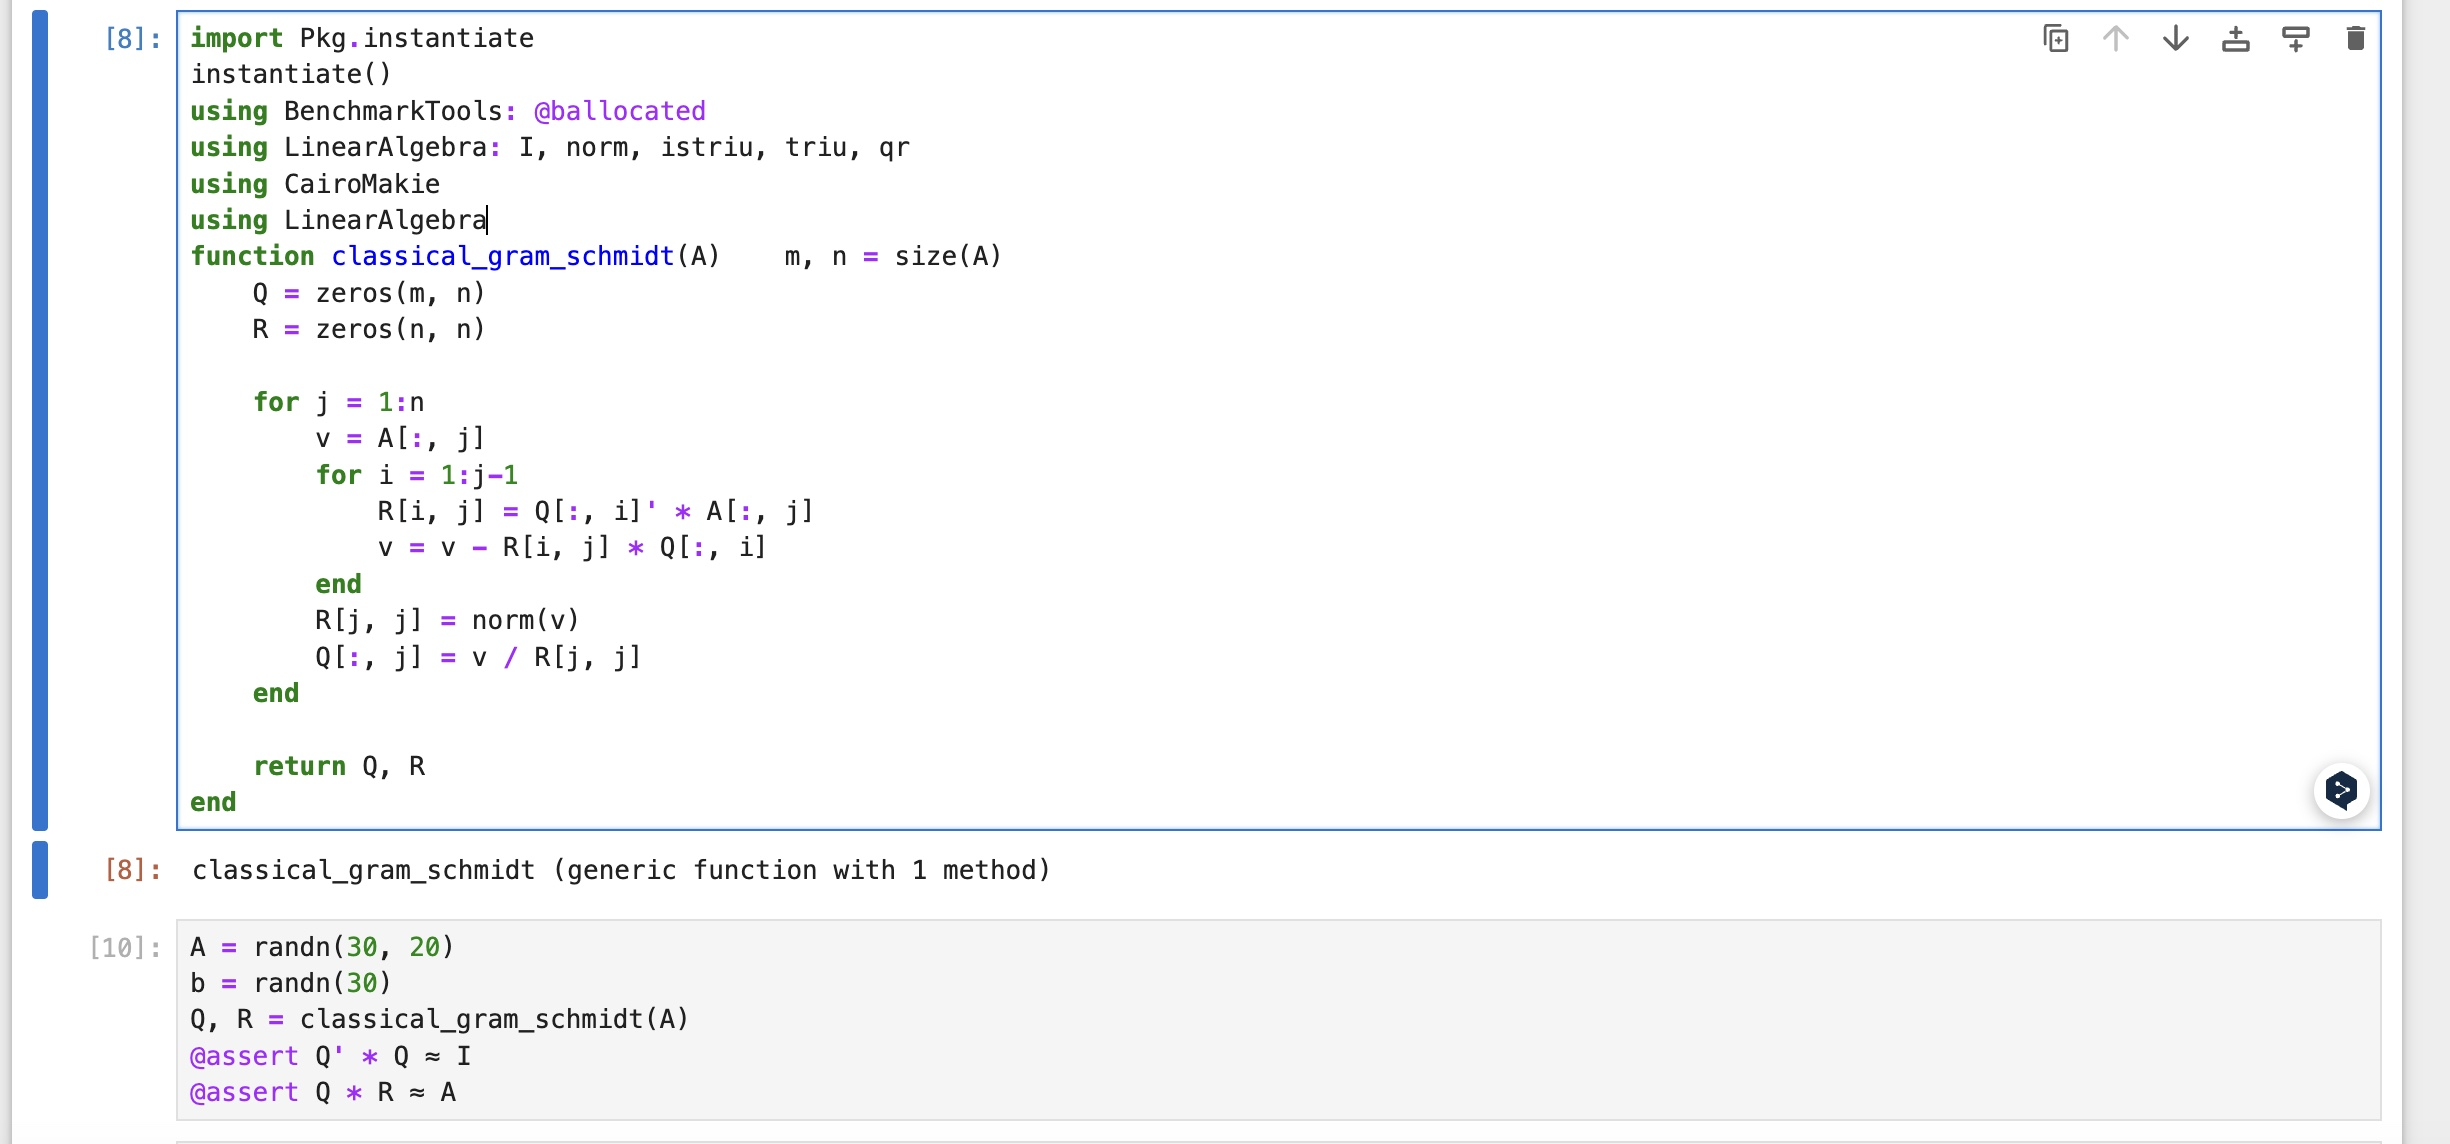
\includegraphics[width=0.75\linewidth]{Image 3-4-24 at 01.22.jpeg}  
\end{figure}
\subsection{(b)}
\begin{minted}{Python}
function modifiedGramSchmidt(A)
    m, n = size(A)
    Q = zeros(m, n)
    R = zeros(n, n)

    for k in 1:n
        v = A[:, k]
        for j in 1:k-1
            R[j, k] = Q[:, j]' * v
            v = v - R[j, k] * Q[:, j]
        end
        R[k, k] = norm(v)
        Q[:, k] = v / R[k, k]
    end

    return Q, R
end

\end{minted}
\begin{figure}[H]
    \centering
    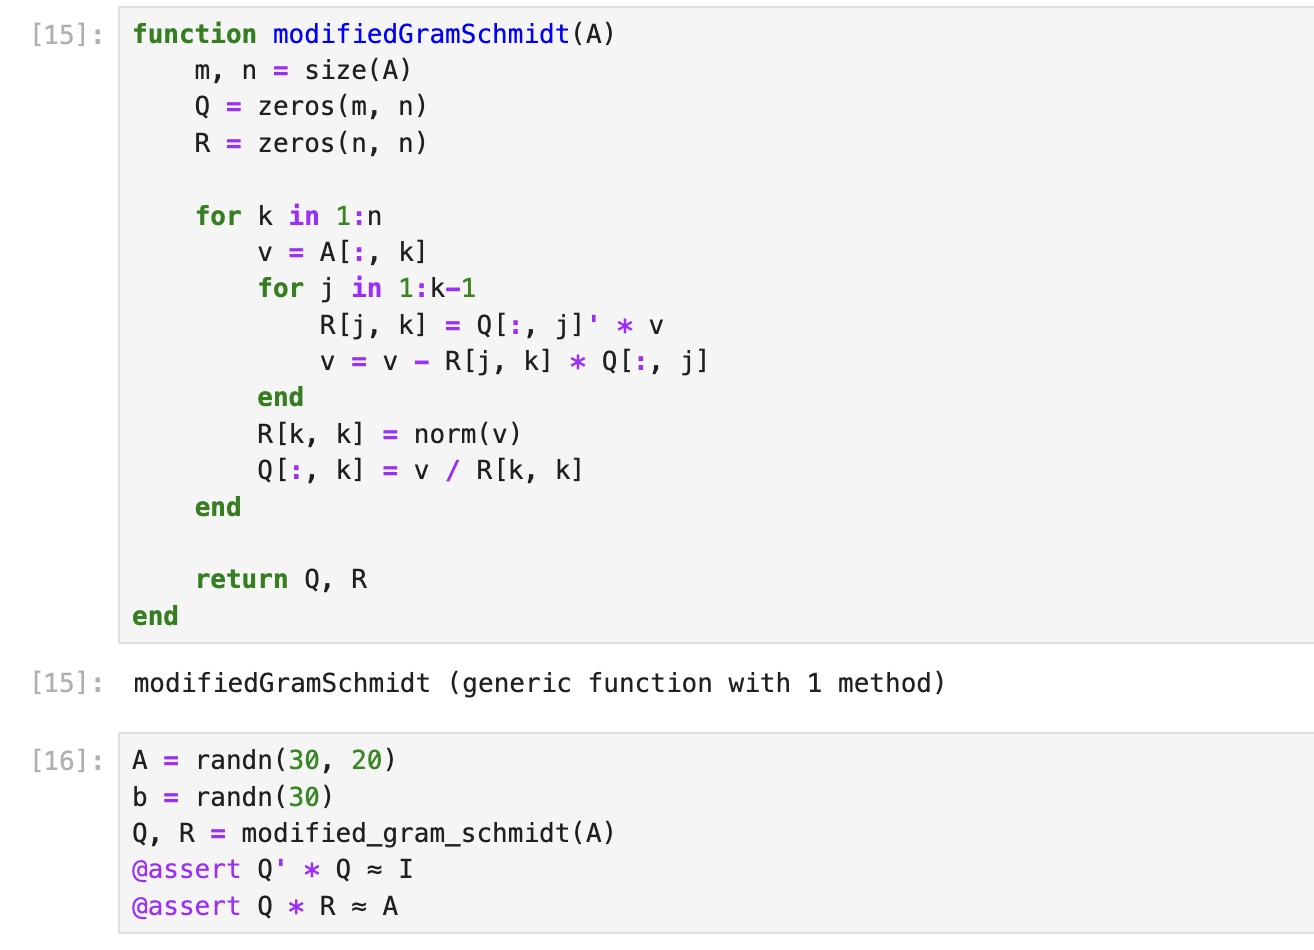
\includegraphics[width=0.75\linewidth]{Image 3-5-24 at 01.01.jpeg}
    
    
\end{figure}
\subsection{(c)}
The function directly modifies A, transforming its upper triangular part into R and storing the essential parts of the Householder vectors in its lower part. The use of in-place updates and avoidance of creating large temporary matrices or vectors are crucial to meet the memory constraint.
The function stores information necessary to reconstruct Q implicitly within the modified parts of A, specifically in its lower triangular part below R.


\begin{minted}{Python}
    function householder_QR!(A)
    m, n = size(A)
    for k in 1:n
        # Identify the subvector to eliminate
        x = A[k:m, k]
        
        # Compute the Householder vector
        v = copy(x)
        v[1] += sign(x[1]) * norm(x)
        v /= norm(v)
        
        # Apply the Householder reflection in-place
        for j in k:n
            A[k:m, j] -= 2 * v * (v' * A[k:m, j])
        end
        
        # Store the Householder vector in A below the diagonal
        A[k+1:m, k] = v[2:end]
    end
    # Zero out below-diagonal elements to enforce R's upper triangularity
    for i in 2:m, j in 1:min(i-1, n)
        A[i, j] = 0
    end
end


\end{minted}
However, it still somehow causes memory allocation.
\begin{figure}[H]
    \centering
    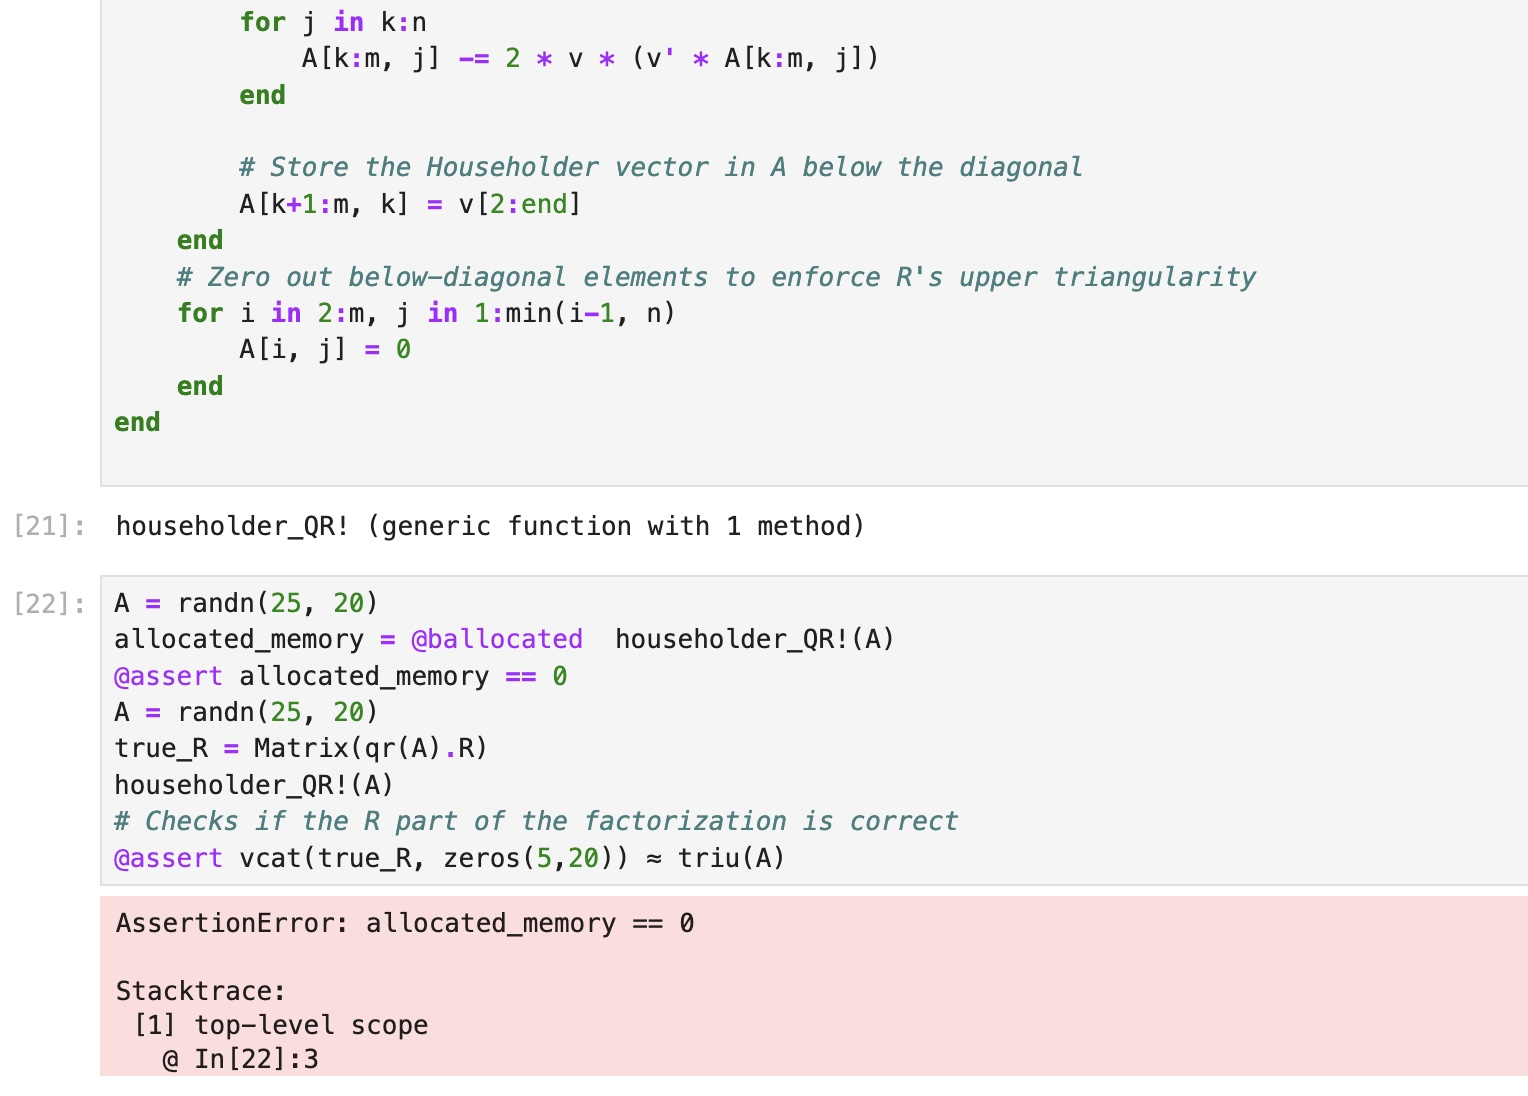
\includegraphics[width=0.75\linewidth]{Image 3-5-24 at 01.09.jpeg}
\end{figure}
\subsection{(d)}
\begin{minted}{Python}
    function householder_QR_mul!(out, x, QR)
    m, n = size(QR)
    # Assume out has been correctly initialized outside this function
    
    for i = 1:n
        beta = 2 / (1 + sum(@view(QR[i+1:end, i]) .^ 2))
        tau = beta * dot(@view(QR[i:end, i]), @view(out[i:end]))
        
        for j = i:m
            out[j] -= tau * (j == i ? 1 : QR[j, i])
        end
    end
end

function householder_QR_div!(out, b, QR)
    m, n = size(QR)
    
    # Apply Q' to b without creating new arrays
    for i = 1:n
        # Directly calculate beta using elements of QR
        beta = 2 / (1 + sum(@view(QR[i+1:end, i]) .^ 2))
        tau = beta * dot(@view(QR[i:end, i]), @view(b[i:end]))
        
        # Adjust b in-place
        b[i] -= tau
        for j = i+1:m
            b[j] -= tau * QR[j, i]
        end
    end
    
    # Solve Rx = Q'b in-place
    for i = n:-1:1
        b[i] /= QR[i, i]
        for j = i-1:-1:1
            b[j] -= QR[j, i] * b[i]
        end
    end
    
    # Copy the result to out
    out .= @view(b[1:n])
end
\end{minted}
The same problem was faced in (d):
\begin{figure}[H]
    \centering
    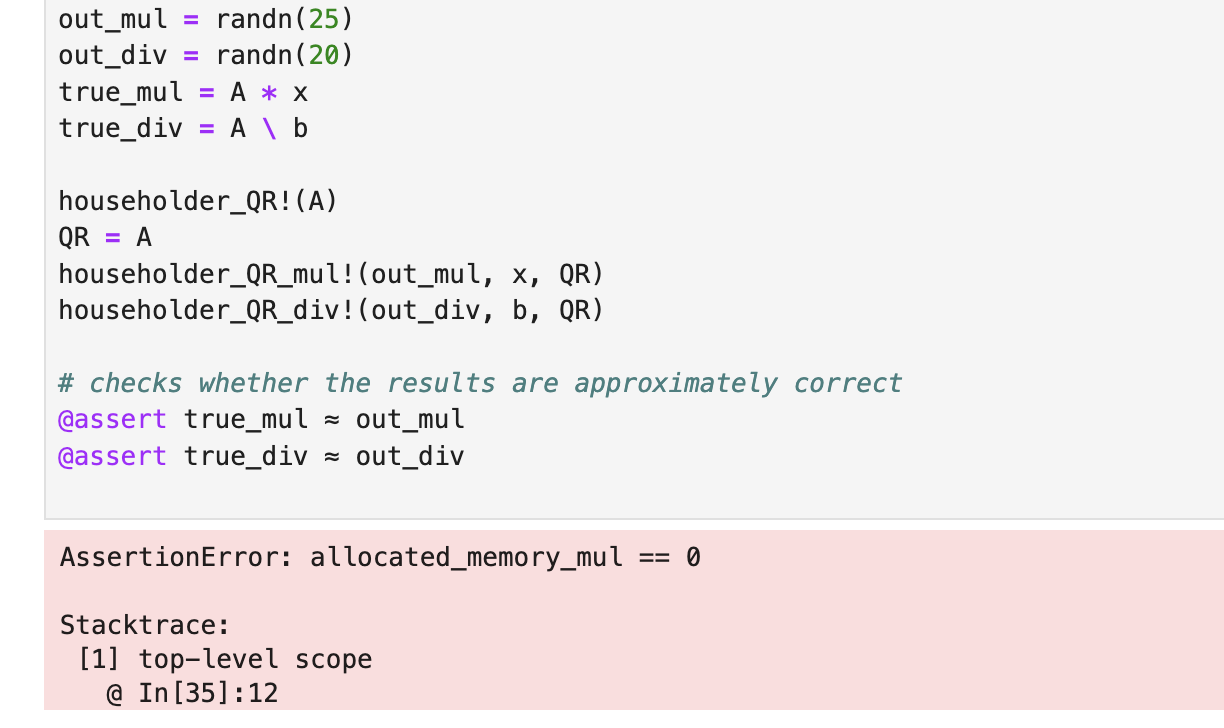
\includegraphics[width=0.75\linewidth]{Screenshot 2024-03-05 at 01.22.17.png}
    
\end{figure}
\subsection{(e)}
\begin{figure}[H]
    \centering
    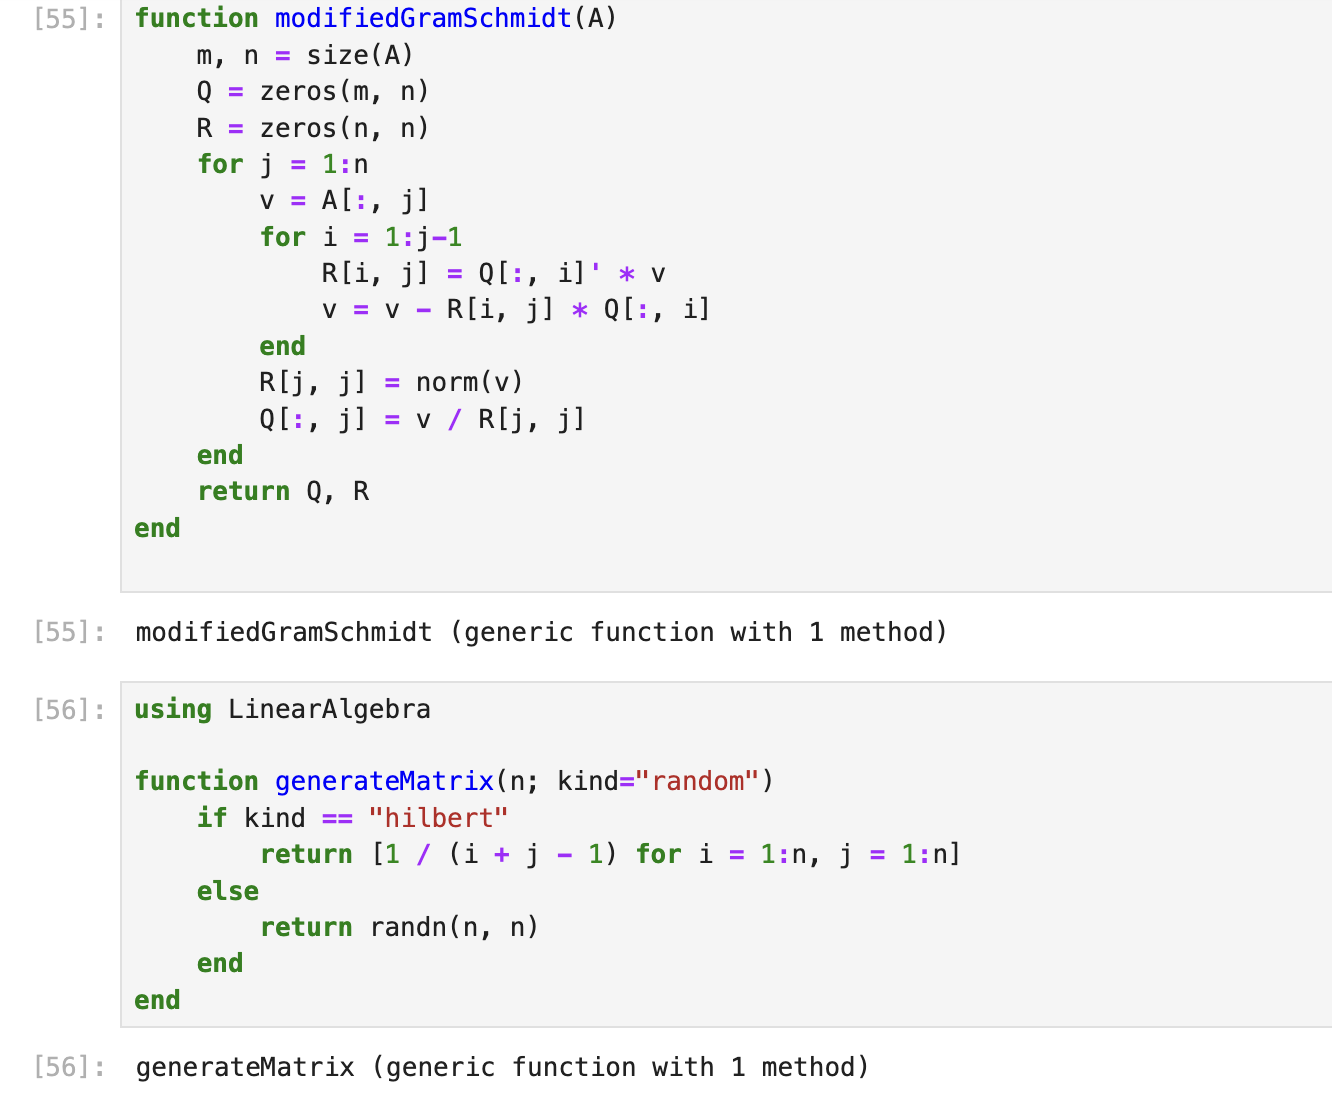
\includegraphics[width=0.75\linewidth]{Screenshot 2024-03-05 at 01.37.13.png}
    
    
\end{figure}
\begin{figure}[H]
    \centering
    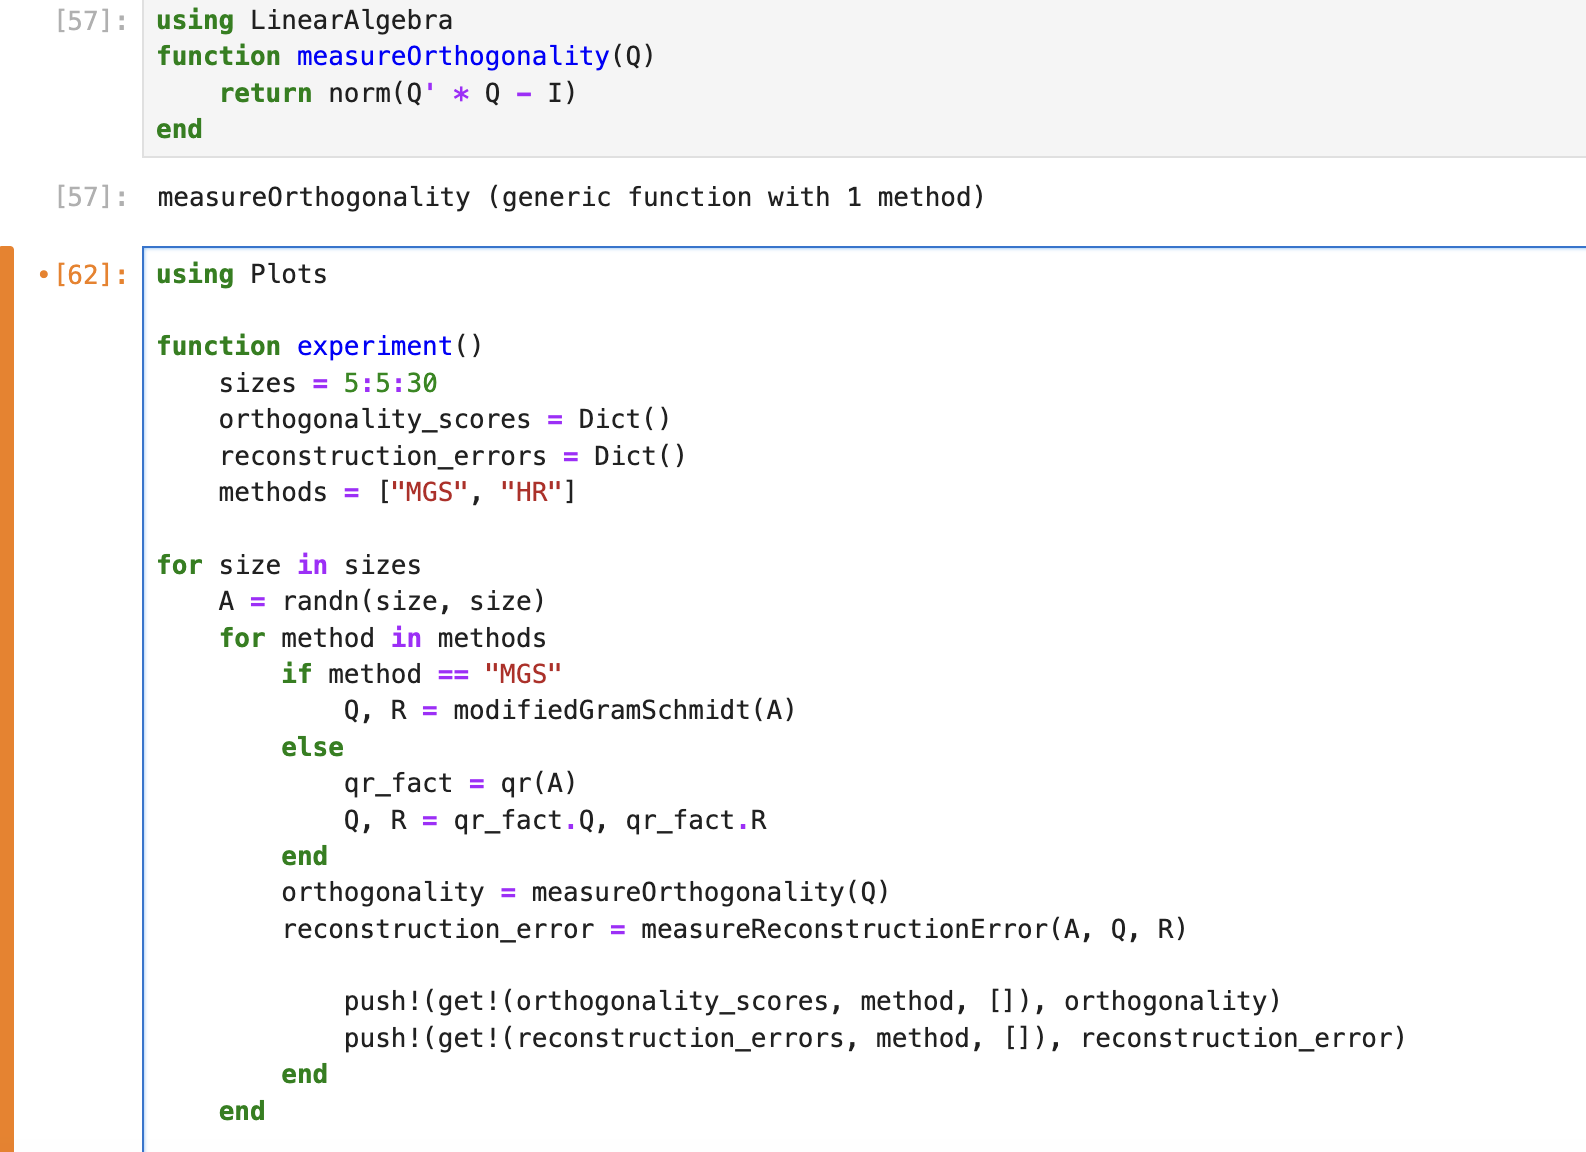
\includegraphics[width=0.75\linewidth]{Screenshot 2024-03-05 at 01.37.39.png}
    
    
\end{figure}
\begin{figure}[H]
    \centering
    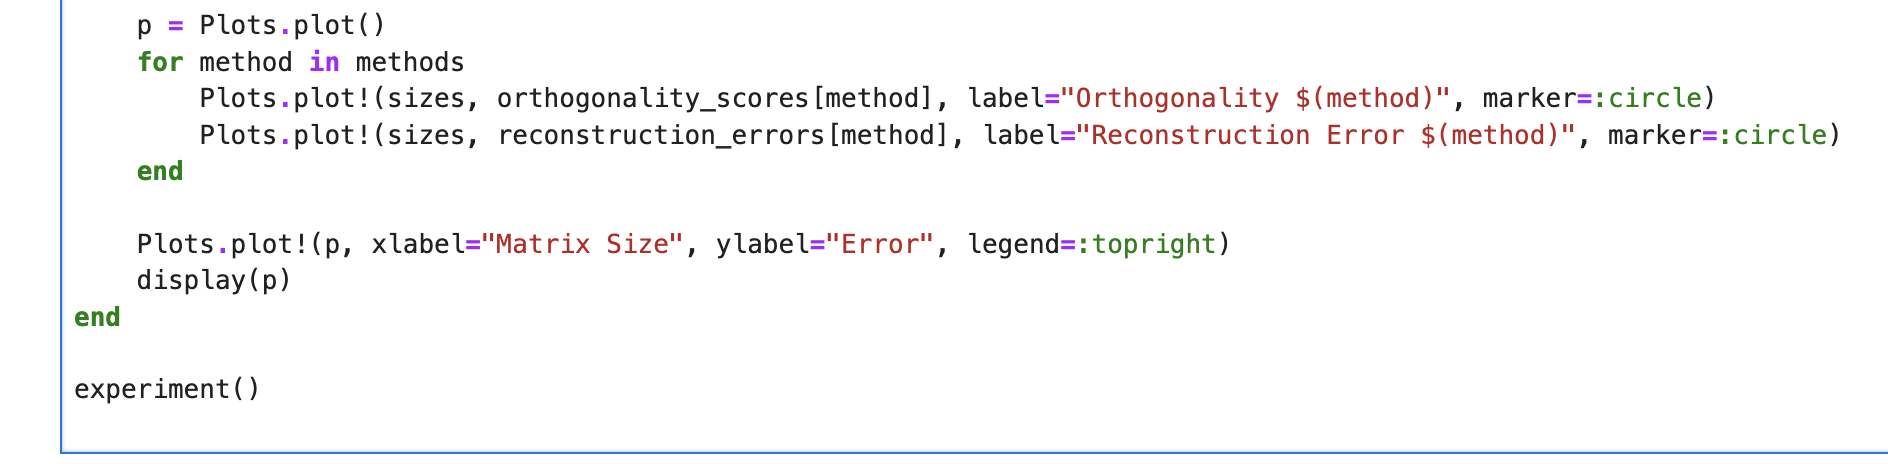
\includegraphics[width=0.75\linewidth]{Screenshot 2024-03-05 at 01.37.59.png}
    
    
\end{figure}
\textbf{The final result is shown as follow:}
\begin{figure}[H]
\centering
    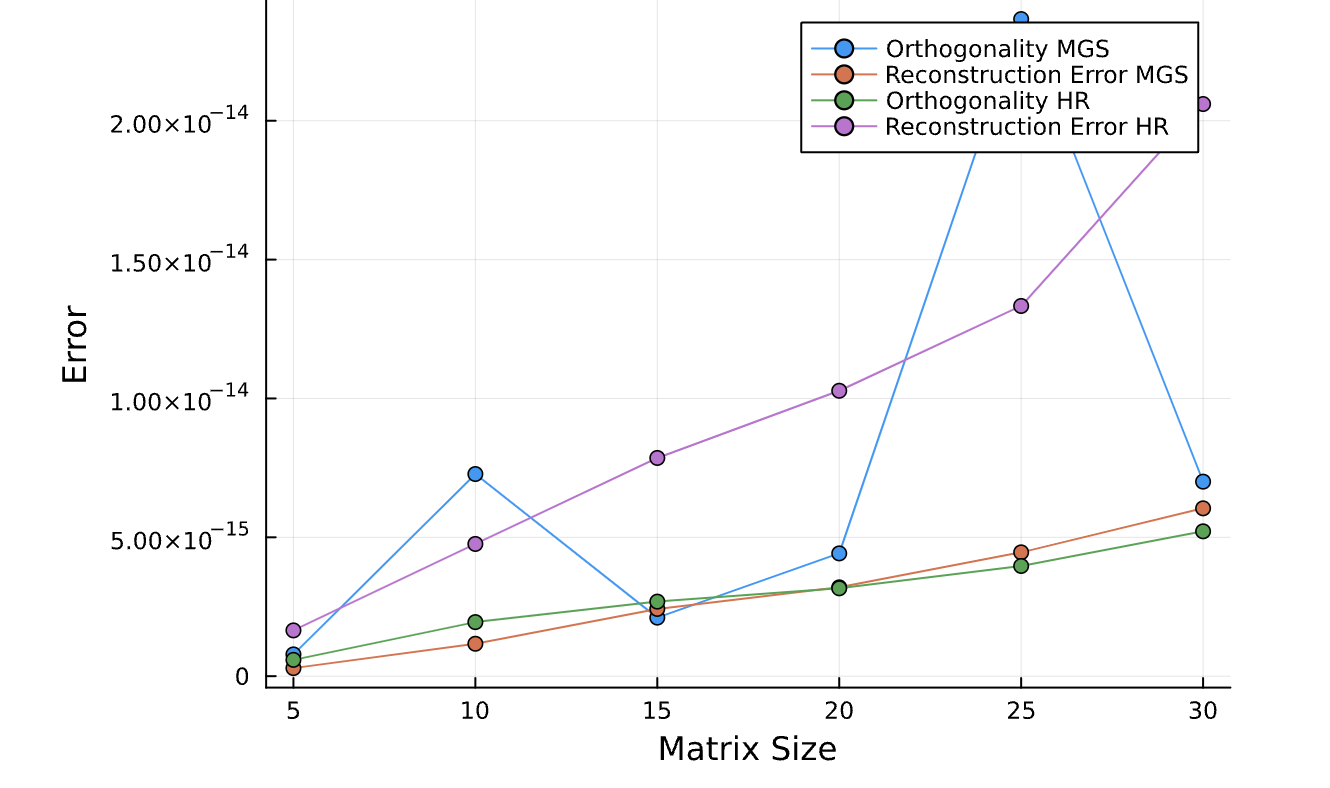
\includegraphics[width=0.75\linewidth]{Screenshot 2024-03-05 at 01.36.41.png}  
\end{figure}
\end{document}